\documentclass[a4paper]{book}
\usepackage{a4wide}
\usepackage{makeidx}
\usepackage{graphicx}
\usepackage{multicol}
\usepackage{float}
\usepackage{listings}
\usepackage{color}
\usepackage{textcomp}
\usepackage{alltt}
\usepackage{times}
\usepackage{ifpdf}
\ifpdf
\usepackage[pdftex,
            pagebackref=true,
            colorlinks=true,
            linkcolor=blue,
            unicode
           ]{hyperref}
\else
\usepackage[ps2pdf,
            pagebackref=true,
            colorlinks=true,
            linkcolor=blue,
            unicode
           ]{hyperref}
\usepackage{pspicture}
\fi
\usepackage[utf8]{inputenc}
\usepackage{doxygen}
\lstset{language=C++,inputencoding=utf8,basicstyle=\footnotesize,breaklines=true,breakatwhitespace=true,tabsize=8,numbers=left }
\makeindex
\setcounter{tocdepth}{3}
\renewcommand{\footrulewidth}{0.4pt}
\begin{document}
\hypersetup{pageanchor=false}
\begin{titlepage}
\vspace*{7cm}
\begin{center}
{\Large GingaWaC }\\
\vspace*{1cm}
{\large Generated by Doxygen 1.6.1}\\
\vspace*{0.5cm}
{\small Mon Feb 1 15:21:19 2010}\\
\end{center}
\end{titlepage}
\clearemptydoublepage
\pagenumbering{roman}
\tableofcontents
\clearemptydoublepage
\pagenumbering{arabic}
\hypersetup{pageanchor=true}
\chapter{Class Index}
\section{Data Structures}
Here are the data structures with brief descriptions:\begin{DoxyCompactList}
\item\contentsline{section}{\hyperlink{classbr_1_1ufscar_1_1lince_1_1ginga_1_1wac_1_1editing_1_1ClientEditingManager}{br::ufscar::lince::ginga::wac::editing::ClientEditingManager} (Permite a aplicações desenvolvidas pelo usuário realizar anotações e edições ao vivo em um documento NCL Esta classe basicamente facilita a criação de aplicações de anotação e edição ao vivo do lado cliente, pois faz parte das tarefas necessárias para aplicações deste tipo, além de permitir retroceder de alterações erroneas e fazer um log das alterações )}{\pageref{classbr_1_1ufscar_1_1lince_1_1ginga_1_1wac_1_1editing_1_1ClientEditingManager}}{}
\item\contentsline{section}{\hyperlink{classbr_1_1ufscar_1_1lince_1_1ginga_1_1wac_1_1editing_1_1EditingCommand}{br::ufscar::lince::ginga::wac::editing::EditingCommand} (Classe que encapsula comandos de edição ao vivo do usuário )}{\pageref{classbr_1_1ufscar_1_1lince_1_1ginga_1_1wac_1_1editing_1_1EditingCommand}}{}
\item\contentsline{section}{\hyperlink{classbr_1_1ufscar_1_1lince_1_1ginga_1_1wac_1_1editing_1_1IClientEditing}{br::ufscar::lince::ginga::wac::editing::IClientEditing} (Interface utilizada pelas aplicações do cliente para utilizar os serviçõs do módulo ClientEditig )}{\pageref{classbr_1_1ufscar_1_1lince_1_1ginga_1_1wac_1_1editing_1_1IClientEditing}}{}
\item\contentsline{section}{\hyperlink{classbr_1_1ufscar_1_1lince_1_1ginga_1_1wac_1_1editing_1_1IFormatterAdapter}{br::ufscar::lince::ginga::wac::editing::IFormatterAdapter} (Interface que permite que as classes do módulo Wac-\/Editing enviem mensagem a classe Formatter do módulo Formatter )}{\pageref{classbr_1_1ufscar_1_1lince_1_1ginga_1_1wac_1_1editing_1_1IFormatterAdapter}}{}
\item\contentsline{section}{\hyperlink{classbr_1_1ufscar_1_1lince_1_1ginga_1_1wac_1_1editing_1_1ILinkAction}{br::ufscar::lince::ginga::wac::editing::ILinkAction} (Interface pela qual é possivel obter informações sobre os links do módulo Formatter )}{\pageref{classbr_1_1ufscar_1_1lince_1_1ginga_1_1wac_1_1editing_1_1ILinkAction}}{}
\item\contentsline{section}{\hyperlink{classbr_1_1ufscar_1_1lince_1_1ginga_1_1wac_1_1editing_1_1IMode}{br::ufscar::lince::ginga::wac::editing::IMode} (Interface que permite a manipulação dos modos de exibição )}{\pageref{classbr_1_1ufscar_1_1lince_1_1ginga_1_1wac_1_1editing_1_1IMode}}{}
\item\contentsline{section}{\hyperlink{classbr_1_1ufscar_1_1lince_1_1ginga_1_1wac_1_1editing_1_1IObjectMode}{br::ufscar::lince::ginga::wac::editing::IObjectMode} (Interface que permite ao módulo Wac-\/Editing Manipular ExecutionObjetcs do módulo Formatter )}{\pageref{classbr_1_1ufscar_1_1lince_1_1ginga_1_1wac_1_1editing_1_1IObjectMode}}{}
\item\contentsline{section}{\hyperlink{classbr_1_1ufscar_1_1lince_1_1ginga_1_1wac_1_1editing_1_1ISchedulerAdapter}{br::ufscar::lince::ginga::wac::editing::ISchedulerAdapter} (Interface pela qual este módulo envia mensagem a classe Scheduler do módulo Formatter )}{\pageref{classbr_1_1ufscar_1_1lince_1_1ginga_1_1wac_1_1editing_1_1ISchedulerAdapter}}{}
\item\contentsline{section}{\hyperlink{classbr_1_1ufscar_1_1lince_1_1ginga_1_1wac_1_1editing_1_1ModeManager}{br::ufscar::lince::ginga::wac::editing::ModeManager} (Classe responsável manipular os modos de exibição do cliente e da emissora )}{\pageref{classbr_1_1ufscar_1_1lince_1_1ginga_1_1wac_1_1editing_1_1ModeManager}}{}
\end{DoxyCompactList}

\chapter{File Index}
\section{File List}
Here is a list of all files with brief descriptions:\begin{DoxyCompactList}
\item\contentsline{section}{include/\hyperlink{INclGenerator_8h}{INclGenerator.h} }{\pageref{INclGenerator_8h}}{}
\item\contentsline{section}{include/\hyperlink{NclFileGenerator_8h}{NclFileGenerator.h} }{\pageref{NclFileGenerator_8h}}{}
\item\contentsline{section}{include/\hyperlink{NclGenerator_8h}{NclGenerator.h} }{\pageref{NclGenerator_8h}}{}
\item\contentsline{section}{include/\hyperlink{UnsupportedNclEntityException_8h}{UnsupportedNclEntityException.h} }{\pageref{UnsupportedNclEntityException_8h}}{}
\item\contentsline{section}{include/generables/\hyperlink{AnchorGenerator_8h}{AnchorGenerator.h} }{\pageref{AnchorGenerator_8h}}{}
\item\contentsline{section}{include/generables/\hyperlink{AssessmentStatementGenerator_8h}{AssessmentStatementGenerator.h} }{\pageref{AssessmentStatementGenerator_8h}}{}
\item\contentsline{section}{include/generables/\hyperlink{AttributeAssessmentGenerator_8h}{AttributeAssessmentGenerator.h} }{\pageref{AttributeAssessmentGenerator_8h}}{}
\item\contentsline{section}{include/generables/\hyperlink{BindGenerator_8h}{BindGenerator.h} }{\pageref{BindGenerator_8h}}{}
\item\contentsline{section}{include/generables/\hyperlink{CausalConnectorGenerator_8h}{CausalConnectorGenerator.h} }{\pageref{CausalConnectorGenerator_8h}}{}
\item\contentsline{section}{include/generables/\hyperlink{CausalLinkGenerator_8h}{CausalLinkGenerator.h} }{\pageref{CausalLinkGenerator_8h}}{}
\item\contentsline{section}{include/generables/\hyperlink{CircleSpatialAnchorGenerator_8h}{CircleSpatialAnchorGenerator.h} }{\pageref{CircleSpatialAnchorGenerator_8h}}{}
\item\contentsline{section}{include/generables/\hyperlink{CompositeRuleGenerator_8h}{CompositeRuleGenerator.h} }{\pageref{CompositeRuleGenerator_8h}}{}
\item\contentsline{section}{include/generables/\hyperlink{CompoundActionGenerator_8h}{CompoundActionGenerator.h} }{\pageref{CompoundActionGenerator_8h}}{}
\item\contentsline{section}{include/generables/\hyperlink{CompoundConditionGenerator_8h}{CompoundConditionGenerator.h} }{\pageref{CompoundConditionGenerator_8h}}{}
\item\contentsline{section}{include/generables/\hyperlink{CompoundStatementGenerator_8h}{CompoundStatementGenerator.h} }{\pageref{CompoundStatementGenerator_8h}}{}
\item\contentsline{section}{include/generables/\hyperlink{ConnectorBaseGenerator_8h}{ConnectorBaseGenerator.h} }{\pageref{ConnectorBaseGenerator_8h}}{}
\item\contentsline{section}{include/generables/\hyperlink{ContentNodeGenerator_8h}{ContentNodeGenerator.h} }{\pageref{ContentNodeGenerator_8h}}{}
\item\contentsline{section}{include/generables/\hyperlink{ContextNodeGenerator_8h}{ContextNodeGenerator.h} }{\pageref{ContextNodeGenerator_8h}}{}
\item\contentsline{section}{include/generables/\hyperlink{DescriptorBaseGenerator_8h}{DescriptorBaseGenerator.h} }{\pageref{DescriptorBaseGenerator_8h}}{}
\item\contentsline{section}{include/generables/\hyperlink{DescriptorGenerator_8h}{DescriptorGenerator.h} }{\pageref{DescriptorGenerator_8h}}{}
\item\contentsline{section}{include/generables/\hyperlink{DescriptorSwitchGenerator_8h}{DescriptorSwitchGenerator.h} }{\pageref{DescriptorSwitchGenerator_8h}}{}
\item\contentsline{section}{include/generables/\hyperlink{Generable_8h}{Generable.h} }{\pageref{Generable_8h}}{}
\item\contentsline{section}{include/generables/\hyperlink{GeneratorUtil_8h}{GeneratorUtil.h} }{\pageref{GeneratorUtil_8h}}{}
\item\contentsline{section}{include/generables/\hyperlink{IntervalAnchorGenerator_8h}{IntervalAnchorGenerator.h} }{\pageref{IntervalAnchorGenerator_8h}}{}
\item\contentsline{section}{include/generables/\hyperlink{LabeledAnchorGenerator_8h}{LabeledAnchorGenerator.h} }{\pageref{LabeledAnchorGenerator_8h}}{}
\item\contentsline{section}{include/generables/\hyperlink{LayoutRegionGenerator_8h}{LayoutRegionGenerator.h} }{\pageref{LayoutRegionGenerator_8h}}{}
\item\contentsline{section}{include/generables/\hyperlink{NclDocumentGenerator_8h}{NclDocumentGenerator.h} }{\pageref{NclDocumentGenerator_8h}}{}
\item\contentsline{section}{include/generables/\hyperlink{ParameterGenerator_8h}{ParameterGenerator.h} }{\pageref{ParameterGenerator_8h}}{}
\item\contentsline{section}{include/generables/\hyperlink{PortGenerator_8h}{PortGenerator.h} }{\pageref{PortGenerator_8h}}{}
\item\contentsline{section}{include/generables/\hyperlink{PropertyAnchorGenerator_8h}{PropertyAnchorGenerator.h} }{\pageref{PropertyAnchorGenerator_8h}}{}
\item\contentsline{section}{include/generables/\hyperlink{RectangleSpatialAnchorGenerator_8h}{RectangleSpatialAnchorGenerator.h} }{\pageref{RectangleSpatialAnchorGenerator_8h}}{}
\item\contentsline{section}{include/generables/\hyperlink{RegionBaseGenerator_8h}{RegionBaseGenerator.h} }{\pageref{RegionBaseGenerator_8h}}{}
\item\contentsline{section}{include/generables/\hyperlink{RuleBaseGenerator_8h}{RuleBaseGenerator.h} }{\pageref{RuleBaseGenerator_8h}}{}
\item\contentsline{section}{include/generables/\hyperlink{SimpleActionGenerator_8h}{SimpleActionGenerator.h} }{\pageref{SimpleActionGenerator_8h}}{}
\item\contentsline{section}{include/generables/\hyperlink{SimpleConditionGenerator_8h}{SimpleConditionGenerator.h} }{\pageref{SimpleConditionGenerator_8h}}{}
\item\contentsline{section}{include/generables/\hyperlink{SimpleRuleGenerator_8h}{SimpleRuleGenerator.h} }{\pageref{SimpleRuleGenerator_8h}}{}
\item\contentsline{section}{include/generables/\hyperlink{SwitchNodeGenerator_8h}{SwitchNodeGenerator.h} }{\pageref{SwitchNodeGenerator_8h}}{}
\item\contentsline{section}{include/generables/\hyperlink{SwitchPortGenerator_8h}{SwitchPortGenerator.h} }{\pageref{SwitchPortGenerator_8h}}{}
\item\contentsline{section}{include/generables/\hyperlink{TextAnchorGenerator_8h}{TextAnchorGenerator.h} }{\pageref{TextAnchorGenerator_8h}}{}
\item\contentsline{section}{include/generables/\hyperlink{TransitionBaseGenerator_8h}{TransitionBaseGenerator.h} }{\pageref{TransitionBaseGenerator_8h}}{}
\item\contentsline{section}{include/generables/\hyperlink{TransitionGenerator_8h}{TransitionGenerator.h} }{\pageref{TransitionGenerator_8h}}{}
\item\contentsline{section}{include/generables/\hyperlink{ValueAssessmentGenerator_8h}{ValueAssessmentGenerator.h} }{\pageref{ValueAssessmentGenerator_8h}}{}
\end{DoxyCompactList}

\chapter{Class Documentation}
\hypertarget{classbr_1_1ufscar_1_1lince_1_1ginga_1_1wac_1_1state_1_1IPlayerWac}{
\section{br::ufscar::lince::ginga::wac::state::IPlayerWac Class Reference}
\label{classbr_1_1ufscar_1_1lince_1_1ginga_1_1wac_1_1state_1_1IPlayerWac}\index{br::ufscar::lince::ginga::wac::state::IPlayerWac@{br::ufscar::lince::ginga::wac::state::IPlayerWac}}
}


Interface utilizada para se obter o PlayerState das classes Players do módulo Formatter.  


{\ttfamily \#include $<$IPlayerWac.h$>$}\subsection*{Public Member Functions}
\begin{DoxyCompactItemize}
\item 
virtual PlayerState $\ast$ \hyperlink{classbr_1_1ufscar_1_1lince_1_1ginga_1_1wac_1_1state_1_1IPlayerWac_afcadf166ea36150534a0bfa037a384c0}{getPlayerState} ()=0
\begin{DoxyCompactList}\small\item\em Retorna o estado atual do player. \item\end{DoxyCompactList}\end{DoxyCompactItemize}


\subsection{Detailed Description}
Interface utilizada para se obter o PlayerState das classes Players do módulo Formatter. Esta interface deve ser implementada pelas classes PlayerAdapter do módulo Formatter do Ginga para que seja possível se obter os estados correntes de cada player em execução. 

\subsection{Member Function Documentation}
\hypertarget{classbr_1_1ufscar_1_1lince_1_1ginga_1_1wac_1_1state_1_1IPlayerWac_afcadf166ea36150534a0bfa037a384c0}{
\index{br::ufscar::lince::ginga::wac::state::IPlayerWac@{br::ufscar::lince::ginga::wac::state::IPlayerWac}!getPlayerState@{getPlayerState}}
\index{getPlayerState@{getPlayerState}!br::ufscar::lince::ginga::wac::state::IPlayerWac@{br::ufscar::lince::ginga::wac::state::IPlayerWac}}
\subsubsection[{getPlayerState}]{\setlength{\rightskip}{0pt plus 5cm}virtual PlayerState$\ast$ br::ufscar::lince::ginga::wac::state::IPlayerWac::getPlayerState ()\hspace{0.3cm}{\ttfamily  \mbox{[}pure virtual\mbox{]}}}}
\label{classbr_1_1ufscar_1_1lince_1_1ginga_1_1wac_1_1state_1_1IPlayerWac_afcadf166ea36150534a0bfa037a384c0}


Retorna o estado atual do player. Instância de PlayerState que contém as informações do estado atual do player. 

The documentation for this class was generated from the following file:\begin{DoxyCompactItemize}
\item 
\hyperlink{IPlayerWac_8h}{IPlayerWac.h}\end{DoxyCompactItemize}

\hypertarget{classbr_1_1ufscar_1_1lince_1_1ginga_1_1wac_1_1state_1_1PlayerStateWac}{
\section{br::ufscar::lince::ginga::wac::state::PlayerStateWac Class Reference}
\label{classbr_1_1ufscar_1_1lince_1_1ginga_1_1wac_1_1state_1_1PlayerStateWac}\index{br::ufscar::lince::ginga::wac::state::PlayerStateWac@{br::ufscar::lince::ginga::wac::state::PlayerStateWac}}
}


Representa o Estado de um Player em um determinado momento.  


{\ttfamily \#include $<$PlayerStateWac.h$>$}\subsection*{Public Member Functions}
\begin{DoxyCompactItemize}
\item 
\hypertarget{classbr_1_1ufscar_1_1lince_1_1ginga_1_1wac_1_1state_1_1PlayerStateWac_aa4757cabc74e55dc316743bba409406c}{
\hyperlink{classbr_1_1ufscar_1_1lince_1_1ginga_1_1wac_1_1state_1_1PlayerStateWac_aa4757cabc74e55dc316743bba409406c}{PlayerStateWac} ()}
\label{classbr_1_1ufscar_1_1lince_1_1ginga_1_1wac_1_1state_1_1PlayerStateWac_aa4757cabc74e55dc316743bba409406c}

\begin{DoxyCompactList}\small\item\em Constrói uma instância de \hyperlink{classbr_1_1ufscar_1_1lince_1_1ginga_1_1wac_1_1state_1_1PlayerStateWac}{PlayerStateWac}. \item\end{DoxyCompactList}\end{DoxyCompactItemize}
\subsection*{Static Public Attributes}
\begin{DoxyCompactItemize}
\item 
\hypertarget{classbr_1_1ufscar_1_1lince_1_1ginga_1_1wac_1_1state_1_1PlayerStateWac_a6a170a55a6826b9b9adf36421f778918}{
static const short \hyperlink{classbr_1_1ufscar_1_1lince_1_1ginga_1_1wac_1_1state_1_1PlayerStateWac_a6a170a55a6826b9b9adf36421f778918}{NONE}}
\label{classbr_1_1ufscar_1_1lince_1_1ginga_1_1wac_1_1state_1_1PlayerStateWac_a6a170a55a6826b9b9adf36421f778918}

\begin{DoxyCompactList}\small\item\em Constante que representa o estado \char`\"{}nenhum\char`\"{} do player. \item\end{DoxyCompactList}\item 
\hypertarget{classbr_1_1ufscar_1_1lince_1_1ginga_1_1wac_1_1state_1_1PlayerStateWac_a199432f24d53a1dbe27bd37df0fc08d9}{
static const short \hyperlink{classbr_1_1ufscar_1_1lince_1_1ginga_1_1wac_1_1state_1_1PlayerStateWac_a199432f24d53a1dbe27bd37df0fc08d9}{PLAY}}
\label{classbr_1_1ufscar_1_1lince_1_1ginga_1_1wac_1_1state_1_1PlayerStateWac_a199432f24d53a1dbe27bd37df0fc08d9}

\begin{DoxyCompactList}\small\item\em Constante que representa o estado \char`\"{}em execução\char`\"{} do player. \item\end{DoxyCompactList}\item 
\hypertarget{classbr_1_1ufscar_1_1lince_1_1ginga_1_1wac_1_1state_1_1PlayerStateWac_af20c4a1c6e1c5ca186a0e868e969bd7d}{
static const short \hyperlink{classbr_1_1ufscar_1_1lince_1_1ginga_1_1wac_1_1state_1_1PlayerStateWac_af20c4a1c6e1c5ca186a0e868e969bd7d}{PAUSE}}
\label{classbr_1_1ufscar_1_1lince_1_1ginga_1_1wac_1_1state_1_1PlayerStateWac_af20c4a1c6e1c5ca186a0e868e969bd7d}

\begin{DoxyCompactList}\small\item\em Constante que representa o estado \char`\"{}pausado\char`\"{} do player. \item\end{DoxyCompactList}\item 
\hypertarget{classbr_1_1ufscar_1_1lince_1_1ginga_1_1wac_1_1state_1_1PlayerStateWac_af8b72d234c4078f41fd2e762a1980806}{
static const short \hyperlink{classbr_1_1ufscar_1_1lince_1_1ginga_1_1wac_1_1state_1_1PlayerStateWac_af8b72d234c4078f41fd2e762a1980806}{STOP}}
\label{classbr_1_1ufscar_1_1lince_1_1ginga_1_1wac_1_1state_1_1PlayerStateWac_af8b72d234c4078f41fd2e762a1980806}

\begin{DoxyCompactList}\small\item\em Constante que representa o estado \char`\"{}parado\char`\"{} do player. \item\end{DoxyCompactList}\end{DoxyCompactItemize}


\subsection{Detailed Description}
Representa o Estado de um Player em um determinado momento. Esta extende a classe PlayerState do módulo gingacc-\/players, possuindo todas as suas funcionalidades. Futuramente, ela pode ser espandida para armazenar mais informações referentes ao estado do player que não podem ser obtidas diretamente da módulo players, mas sim da classe PlayerAdapter do módulo Formatter. 

The documentation for this class was generated from the following file:\begin{DoxyCompactItemize}
\item 
\hyperlink{PlayerStateWac_8h}{PlayerStateWac.h}\end{DoxyCompactItemize}

\hypertarget{classbr_1_1ufscar_1_1lince_1_1ginga_1_1wac_1_1state_1_1PresentationState}{
\section{br::ufscar::lince::ginga::wac::state::PresentationState Class Reference}
\label{classbr_1_1ufscar_1_1lince_1_1ginga_1_1wac_1_1state_1_1PresentationState}\index{br::ufscar::lince::ginga::wac::state::PresentationState@{br::ufscar::lince::ginga::wac::state::PresentationState}}
}


Representa o estado da apresentação como um todo em um dado momento.  




{\ttfamily \#include $<$PresentationState.h$>$}

Inheritance diagram for br::ufscar::lince::ginga::wac::state::PresentationState:\begin{figure}[H]
\begin{center}
\leavevmode
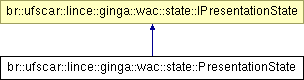
\includegraphics[height=2cm]{classbr_1_1ufscar_1_1lince_1_1ginga_1_1wac_1_1state_1_1PresentationState}
\end{center}
\end{figure}
\subsection*{Public Member Functions}
\begin{DoxyCompactItemize}
\item 
\hyperlink{classbr_1_1ufscar_1_1lince_1_1ginga_1_1wac_1_1state_1_1PresentationState_aa48f61ac6a0cf382182bd6fb4f548b87}{PresentationState} ()
\begin{DoxyCompactList}\small\item\em Constrói uma instância de \hyperlink{classbr_1_1ufscar_1_1lince_1_1ginga_1_1wac_1_1state_1_1PresentationState}{PresentationState}. \item\end{DoxyCompactList}\item 
\hyperlink{classbr_1_1ufscar_1_1lince_1_1ginga_1_1wac_1_1state_1_1PresentationState_a324581a9a822f53cf7365321ae35f2ec}{$\sim$PresentationState} ()
\begin{DoxyCompactList}\small\item\em Destrói a instância de \hyperlink{classbr_1_1ufscar_1_1lince_1_1ginga_1_1wac_1_1state_1_1PresentationState}{PresentationState}. \item\end{DoxyCompactList}\item 
void \hyperlink{classbr_1_1ufscar_1_1lince_1_1ginga_1_1wac_1_1state_1_1PresentationState_a02bf97b60acc4e5ba168961d8e695195}{setStateMap} (map$<$ string, \hyperlink{classbr_1_1ufscar_1_1lince_1_1ginga_1_1wac_1_1state_1_1IElementaryState}{IElementaryState} $\ast$ $>$ $\ast$nStateMap, map$<$ string, string $>$ $\ast$nDescMap, map$<$ string, string $>$ $\ast$nContextMap)
\begin{DoxyCompactList}\small\item\em Seta os mapas que contém os estados dos players da apresentação. \item\end{DoxyCompactList}\item 
void \hyperlink{classbr_1_1ufscar_1_1lince_1_1ginga_1_1wac_1_1state_1_1PresentationState_aadc7632e1bff7b0c2680a5193679e1d9}{setDcoumentName} (string name)
\begin{DoxyCompactList}\small\item\em Seta o nome do documento NCL. \item\end{DoxyCompactList}\item 
void \hyperlink{classbr_1_1ufscar_1_1lince_1_1ginga_1_1wac_1_1state_1_1PresentationState_a127842284622579c23ec1d6ce974fe8f}{setPrivateBaseName} (string name)
\begin{DoxyCompactList}\small\item\em Seta o nome da base privada. \item\end{DoxyCompactList}\item 
virtual vector$<$ string $>$ $\ast$ \hyperlink{classbr_1_1ufscar_1_1lince_1_1ginga_1_1wac_1_1state_1_1PresentationState_a82bc0879c2e2d6c6eb48ffaeee043bac}{getPlayersNames} ()
\begin{DoxyCompactList}\small\item\em Retorna o nome de todos os players da apresentação atual. \item\end{DoxyCompactList}\item 
virtual \hyperlink{classbr_1_1ufscar_1_1lince_1_1ginga_1_1wac_1_1state_1_1IElementaryState}{IElementaryState} $\ast$ \hyperlink{classbr_1_1ufscar_1_1lince_1_1ginga_1_1wac_1_1state_1_1PresentationState_a460f75f353ea3508dacdbd2a29bd537e}{getElementaryState} (string name)
\begin{DoxyCompactList}\small\item\em Retorna o estado de um determinado Player. \item\end{DoxyCompactList}\item 
virtual string \hyperlink{classbr_1_1ufscar_1_1lince_1_1ginga_1_1wac_1_1state_1_1PresentationState_a5f3306aca36ba9aac7c43d27f6f29ad9}{getMediaDescriptor} (string name)
\begin{DoxyCompactList}\small\item\em Retorna o Descritor associado ao nó de mídia de um player. \item\end{DoxyCompactList}\item 
virtual string \hyperlink{classbr_1_1ufscar_1_1lince_1_1ginga_1_1wac_1_1state_1_1PresentationState_af4149387468f9a7180c036f4fdce03bd}{getPresentationName} ()
\begin{DoxyCompactList}\small\item\em Retorna o nome completo da apresentação. \item\end{DoxyCompactList}\item 
virtual string \hyperlink{classbr_1_1ufscar_1_1lince_1_1ginga_1_1wac_1_1state_1_1PresentationState_a90a8797bdaffaed86c5a686652fea889}{getDocumentName} ()
\begin{DoxyCompactList}\small\item\em Retorna o nome do documento NCL. \item\end{DoxyCompactList}\item 
virtual string \hyperlink{classbr_1_1ufscar_1_1lince_1_1ginga_1_1wac_1_1state_1_1PresentationState_a5b280537bd03a744eb41807859f01413}{getPrivateBaseName} ()
\begin{DoxyCompactList}\small\item\em Retorna o nome da base privada. \item\end{DoxyCompactList}\item 
virtual string \hyperlink{classbr_1_1ufscar_1_1lince_1_1ginga_1_1wac_1_1state_1_1PresentationState_a00ec06809774af254532488cc1559c15}{toString} ()
\begin{DoxyCompactList}\small\item\em Retorna uma string contento o resumo das principais informações relativas ao estado da apresentação presentados pelo objeto. \item\end{DoxyCompactList}\item 
virtual vector$<$ string $>$ $\ast$ \hyperlink{classbr_1_1ufscar_1_1lince_1_1ginga_1_1wac_1_1state_1_1PresentationState_ab5f9e22342f390d01e54ca51f8a85609}{getContextPropertyNames} ()
\begin{DoxyCompactList}\small\item\em Este método retorna todos os nomes das propriedades relativas ao contexto da apresentação. \item\end{DoxyCompactList}\item 
virtual string \hyperlink{classbr_1_1ufscar_1_1lince_1_1ginga_1_1wac_1_1state_1_1PresentationState_a2931ba17e6dcd1352382fee289352f4b}{getContextPropertyValue} (string attributeId)
\begin{DoxyCompactList}\small\item\em Este método retorna o valor de uma determinada propriedade do contexto da apresentação através de uma string. \item\end{DoxyCompactList}\end{DoxyCompactItemize}


\subsection{Detailed Description}
Representa o estado da apresentação como um todo em um dado momento. Esta classe agrupa o estado de todos os players de uma apresentação NCL além de outras informações mais gerais da apresentação, representado o estado de uma apresentação NCL em um dado momento. 

\subsection{Constructor \& Destructor Documentation}
\hypertarget{classbr_1_1ufscar_1_1lince_1_1ginga_1_1wac_1_1state_1_1PresentationState_aa48f61ac6a0cf382182bd6fb4f548b87}{
\index{br::ufscar::lince::ginga::wac::state::PresentationState@{br::ufscar::lince::ginga::wac::state::PresentationState}!PresentationState@{PresentationState}}
\index{PresentationState@{PresentationState}!br::ufscar::lince::ginga::wac::state::PresentationState@{br::ufscar::lince::ginga::wac::state::PresentationState}}
\subsubsection[{PresentationState}]{\setlength{\rightskip}{0pt plus 5cm}br::ufscar::lince::ginga::wac::state::PresentationState::PresentationState ()}}
\label{classbr_1_1ufscar_1_1lince_1_1ginga_1_1wac_1_1state_1_1PresentationState_aa48f61ac6a0cf382182bd6fb4f548b87}


Constrói uma instância de \hyperlink{classbr_1_1ufscar_1_1lince_1_1ginga_1_1wac_1_1state_1_1PresentationState}{PresentationState}. 

\hypertarget{classbr_1_1ufscar_1_1lince_1_1ginga_1_1wac_1_1state_1_1PresentationState_a324581a9a822f53cf7365321ae35f2ec}{
\index{br::ufscar::lince::ginga::wac::state::PresentationState@{br::ufscar::lince::ginga::wac::state::PresentationState}!$\sim$PresentationState@{$\sim$PresentationState}}
\index{$\sim$PresentationState@{$\sim$PresentationState}!br::ufscar::lince::ginga::wac::state::PresentationState@{br::ufscar::lince::ginga::wac::state::PresentationState}}
\subsubsection[{$\sim$PresentationState}]{\setlength{\rightskip}{0pt plus 5cm}br::ufscar::lince::ginga::wac::state::PresentationState::$\sim$PresentationState ()}}
\label{classbr_1_1ufscar_1_1lince_1_1ginga_1_1wac_1_1state_1_1PresentationState_a324581a9a822f53cf7365321ae35f2ec}


Destrói a instância de \hyperlink{classbr_1_1ufscar_1_1lince_1_1ginga_1_1wac_1_1state_1_1PresentationState}{PresentationState}. 



\subsection{Member Function Documentation}
\hypertarget{classbr_1_1ufscar_1_1lince_1_1ginga_1_1wac_1_1state_1_1PresentationState_ab5f9e22342f390d01e54ca51f8a85609}{
\index{br::ufscar::lince::ginga::wac::state::PresentationState@{br::ufscar::lince::ginga::wac::state::PresentationState}!getContextPropertyNames@{getContextPropertyNames}}
\index{getContextPropertyNames@{getContextPropertyNames}!br::ufscar::lince::ginga::wac::state::PresentationState@{br::ufscar::lince::ginga::wac::state::PresentationState}}
\subsubsection[{getContextPropertyNames}]{\setlength{\rightskip}{0pt plus 5cm}virtual vector$<$string$>$$\ast$ br::ufscar::lince::ginga::wac::state::PresentationState::getContextPropertyNames ()\hspace{0.3cm}{\ttfamily  \mbox{[}virtual\mbox{]}}}}
\label{classbr_1_1ufscar_1_1lince_1_1ginga_1_1wac_1_1state_1_1PresentationState_ab5f9e22342f390d01e54ca51f8a85609}


Este método retorna todos os nomes das propriedades relativas ao contexto da apresentação. 


\begin{DoxyParams}{Parameters}
\item[{\em Um}]vetor contento o nome das propriedades relativas ao contexto. \end{DoxyParams}


Implements \hyperlink{classbr_1_1ufscar_1_1lince_1_1ginga_1_1wac_1_1state_1_1IPresentationState_a3ec5c1d54f31461e1a3e81a54fefaa87}{br::ufscar::lince::ginga::wac::state::IPresentationState}.

\hypertarget{classbr_1_1ufscar_1_1lince_1_1ginga_1_1wac_1_1state_1_1PresentationState_a2931ba17e6dcd1352382fee289352f4b}{
\index{br::ufscar::lince::ginga::wac::state::PresentationState@{br::ufscar::lince::ginga::wac::state::PresentationState}!getContextPropertyValue@{getContextPropertyValue}}
\index{getContextPropertyValue@{getContextPropertyValue}!br::ufscar::lince::ginga::wac::state::PresentationState@{br::ufscar::lince::ginga::wac::state::PresentationState}}
\subsubsection[{getContextPropertyValue}]{\setlength{\rightskip}{0pt plus 5cm}virtual string br::ufscar::lince::ginga::wac::state::PresentationState::getContextPropertyValue (string {\em attributeId})\hspace{0.3cm}{\ttfamily  \mbox{[}virtual\mbox{]}}}}
\label{classbr_1_1ufscar_1_1lince_1_1ginga_1_1wac_1_1state_1_1PresentationState_a2931ba17e6dcd1352382fee289352f4b}


Este método retorna o valor de uma determinada propriedade do contexto da apresentação através de uma string. 


\begin{DoxyParams}{Parameters}
\item[{\em attributeId}]O identificador da propriedade do contexto. \end{DoxyParams}
\begin{DoxyReturn}{Returns}
O valor da propriedade representada através de uma string 
\end{DoxyReturn}


Implements \hyperlink{classbr_1_1ufscar_1_1lince_1_1ginga_1_1wac_1_1state_1_1IPresentationState_a3d16c8c6c2c90ef84313414072d953cf}{br::ufscar::lince::ginga::wac::state::IPresentationState}.

\hypertarget{classbr_1_1ufscar_1_1lince_1_1ginga_1_1wac_1_1state_1_1PresentationState_a90a8797bdaffaed86c5a686652fea889}{
\index{br::ufscar::lince::ginga::wac::state::PresentationState@{br::ufscar::lince::ginga::wac::state::PresentationState}!getDocumentName@{getDocumentName}}
\index{getDocumentName@{getDocumentName}!br::ufscar::lince::ginga::wac::state::PresentationState@{br::ufscar::lince::ginga::wac::state::PresentationState}}
\subsubsection[{getDocumentName}]{\setlength{\rightskip}{0pt plus 5cm}virtual string br::ufscar::lince::ginga::wac::state::PresentationState::getDocumentName ()\hspace{0.3cm}{\ttfamily  \mbox{[}virtual\mbox{]}}}}
\label{classbr_1_1ufscar_1_1lince_1_1ginga_1_1wac_1_1state_1_1PresentationState_a90a8797bdaffaed86c5a686652fea889}


Retorna o nome do documento NCL. 

\begin{DoxyReturn}{Returns}
String contendo o nome do documento NCL. 
\end{DoxyReturn}


Implements \hyperlink{classbr_1_1ufscar_1_1lince_1_1ginga_1_1wac_1_1state_1_1IPresentationState_a20c06c68a1db0160932abf7d6aa4967c}{br::ufscar::lince::ginga::wac::state::IPresentationState}.

\hypertarget{classbr_1_1ufscar_1_1lince_1_1ginga_1_1wac_1_1state_1_1PresentationState_a460f75f353ea3508dacdbd2a29bd537e}{
\index{br::ufscar::lince::ginga::wac::state::PresentationState@{br::ufscar::lince::ginga::wac::state::PresentationState}!getElementaryState@{getElementaryState}}
\index{getElementaryState@{getElementaryState}!br::ufscar::lince::ginga::wac::state::PresentationState@{br::ufscar::lince::ginga::wac::state::PresentationState}}
\subsubsection[{getElementaryState}]{\setlength{\rightskip}{0pt plus 5cm}virtual {\bf IElementaryState}$\ast$ br::ufscar::lince::ginga::wac::state::PresentationState::getElementaryState (string {\em name})\hspace{0.3cm}{\ttfamily  \mbox{[}virtual\mbox{]}}}}
\label{classbr_1_1ufscar_1_1lince_1_1ginga_1_1wac_1_1state_1_1PresentationState_a460f75f353ea3508dacdbd2a29bd537e}


Retorna o estado de um determinado Player. 


\begin{DoxyParams}{Parameters}
\item[{\em name}]Nome do player o qual se deseja obter o estado. \end{DoxyParams}
\begin{DoxyReturn}{Returns}
Instância de PlayerStateWac com o estado atual do player. 
\end{DoxyReturn}


Implements \hyperlink{classbr_1_1ufscar_1_1lince_1_1ginga_1_1wac_1_1state_1_1IPresentationState_a42e36ac35404e13df2b3df4f2da614a1}{br::ufscar::lince::ginga::wac::state::IPresentationState}.

\hypertarget{classbr_1_1ufscar_1_1lince_1_1ginga_1_1wac_1_1state_1_1PresentationState_a5f3306aca36ba9aac7c43d27f6f29ad9}{
\index{br::ufscar::lince::ginga::wac::state::PresentationState@{br::ufscar::lince::ginga::wac::state::PresentationState}!getMediaDescriptor@{getMediaDescriptor}}
\index{getMediaDescriptor@{getMediaDescriptor}!br::ufscar::lince::ginga::wac::state::PresentationState@{br::ufscar::lince::ginga::wac::state::PresentationState}}
\subsubsection[{getMediaDescriptor}]{\setlength{\rightskip}{0pt plus 5cm}virtual string br::ufscar::lince::ginga::wac::state::PresentationState::getMediaDescriptor (string {\em name})\hspace{0.3cm}{\ttfamily  \mbox{[}virtual\mbox{]}}}}
\label{classbr_1_1ufscar_1_1lince_1_1ginga_1_1wac_1_1state_1_1PresentationState_a5f3306aca36ba9aac7c43d27f6f29ad9}


Retorna o Descritor associado ao nó de mídia de um player. 


\begin{DoxyParams}{Parameters}
\item[{\em Nome}]do Player relacionado ao nó de mídia. \end{DoxyParams}
\begin{DoxyReturn}{Returns}
Nome do descritor associado ao nó de mídia. 
\end{DoxyReturn}


Implements \hyperlink{classbr_1_1ufscar_1_1lince_1_1ginga_1_1wac_1_1state_1_1IPresentationState_a4a8d2526ea16319ea1efc19928ffe028}{br::ufscar::lince::ginga::wac::state::IPresentationState}.

\hypertarget{classbr_1_1ufscar_1_1lince_1_1ginga_1_1wac_1_1state_1_1PresentationState_a82bc0879c2e2d6c6eb48ffaeee043bac}{
\index{br::ufscar::lince::ginga::wac::state::PresentationState@{br::ufscar::lince::ginga::wac::state::PresentationState}!getPlayersNames@{getPlayersNames}}
\index{getPlayersNames@{getPlayersNames}!br::ufscar::lince::ginga::wac::state::PresentationState@{br::ufscar::lince::ginga::wac::state::PresentationState}}
\subsubsection[{getPlayersNames}]{\setlength{\rightskip}{0pt plus 5cm}virtual vector$<$string$>$$\ast$ br::ufscar::lince::ginga::wac::state::PresentationState::getPlayersNames ()\hspace{0.3cm}{\ttfamily  \mbox{[}virtual\mbox{]}}}}
\label{classbr_1_1ufscar_1_1lince_1_1ginga_1_1wac_1_1state_1_1PresentationState_a82bc0879c2e2d6c6eb48ffaeee043bac}


Retorna o nome de todos os players da apresentação atual. 

\begin{DoxyReturn}{Returns}
Instância de vector contendo todos os nomes dos players da apresentação atual. 
\end{DoxyReturn}


Implements \hyperlink{classbr_1_1ufscar_1_1lince_1_1ginga_1_1wac_1_1state_1_1IPresentationState_ac3ba6e82191af041b1bc4320ddaf0ca5}{br::ufscar::lince::ginga::wac::state::IPresentationState}.

\hypertarget{classbr_1_1ufscar_1_1lince_1_1ginga_1_1wac_1_1state_1_1PresentationState_af4149387468f9a7180c036f4fdce03bd}{
\index{br::ufscar::lince::ginga::wac::state::PresentationState@{br::ufscar::lince::ginga::wac::state::PresentationState}!getPresentationName@{getPresentationName}}
\index{getPresentationName@{getPresentationName}!br::ufscar::lince::ginga::wac::state::PresentationState@{br::ufscar::lince::ginga::wac::state::PresentationState}}
\subsubsection[{getPresentationName}]{\setlength{\rightskip}{0pt plus 5cm}virtual string br::ufscar::lince::ginga::wac::state::PresentationState::getPresentationName ()\hspace{0.3cm}{\ttfamily  \mbox{[}virtual\mbox{]}}}}
\label{classbr_1_1ufscar_1_1lince_1_1ginga_1_1wac_1_1state_1_1PresentationState_af4149387468f9a7180c036f4fdce03bd}


Retorna o nome completo da apresentação. 

\begin{DoxyReturn}{Returns}
String contendo o nome completo da apresentação; 
\end{DoxyReturn}


Implements \hyperlink{classbr_1_1ufscar_1_1lince_1_1ginga_1_1wac_1_1state_1_1IPresentationState_a939e322cd15e49680f227bfc6b9ded9d}{br::ufscar::lince::ginga::wac::state::IPresentationState}.

\hypertarget{classbr_1_1ufscar_1_1lince_1_1ginga_1_1wac_1_1state_1_1PresentationState_a5b280537bd03a744eb41807859f01413}{
\index{br::ufscar::lince::ginga::wac::state::PresentationState@{br::ufscar::lince::ginga::wac::state::PresentationState}!getPrivateBaseName@{getPrivateBaseName}}
\index{getPrivateBaseName@{getPrivateBaseName}!br::ufscar::lince::ginga::wac::state::PresentationState@{br::ufscar::lince::ginga::wac::state::PresentationState}}
\subsubsection[{getPrivateBaseName}]{\setlength{\rightskip}{0pt plus 5cm}virtual string br::ufscar::lince::ginga::wac::state::PresentationState::getPrivateBaseName ()\hspace{0.3cm}{\ttfamily  \mbox{[}virtual\mbox{]}}}}
\label{classbr_1_1ufscar_1_1lince_1_1ginga_1_1wac_1_1state_1_1PresentationState_a5b280537bd03a744eb41807859f01413}


Retorna o nome da base privada. 

\begin{DoxyReturn}{Returns}
String contendo o nome da base privada. 
\end{DoxyReturn}


Implements \hyperlink{classbr_1_1ufscar_1_1lince_1_1ginga_1_1wac_1_1state_1_1IPresentationState_a53e509fcb89622fa57b299526f96f728}{br::ufscar::lince::ginga::wac::state::IPresentationState}.

\hypertarget{classbr_1_1ufscar_1_1lince_1_1ginga_1_1wac_1_1state_1_1PresentationState_aadc7632e1bff7b0c2680a5193679e1d9}{
\index{br::ufscar::lince::ginga::wac::state::PresentationState@{br::ufscar::lince::ginga::wac::state::PresentationState}!setDcoumentName@{setDcoumentName}}
\index{setDcoumentName@{setDcoumentName}!br::ufscar::lince::ginga::wac::state::PresentationState@{br::ufscar::lince::ginga::wac::state::PresentationState}}
\subsubsection[{setDcoumentName}]{\setlength{\rightskip}{0pt plus 5cm}void br::ufscar::lince::ginga::wac::state::PresentationState::setDcoumentName (string {\em name})}}
\label{classbr_1_1ufscar_1_1lince_1_1ginga_1_1wac_1_1state_1_1PresentationState_aadc7632e1bff7b0c2680a5193679e1d9}


Seta o nome do documento NCL. 


\begin{DoxyParams}{Parameters}
\item[{\em name}]Nome do documento NCL. \end{DoxyParams}
\hypertarget{classbr_1_1ufscar_1_1lince_1_1ginga_1_1wac_1_1state_1_1PresentationState_a127842284622579c23ec1d6ce974fe8f}{
\index{br::ufscar::lince::ginga::wac::state::PresentationState@{br::ufscar::lince::ginga::wac::state::PresentationState}!setPrivateBaseName@{setPrivateBaseName}}
\index{setPrivateBaseName@{setPrivateBaseName}!br::ufscar::lince::ginga::wac::state::PresentationState@{br::ufscar::lince::ginga::wac::state::PresentationState}}
\subsubsection[{setPrivateBaseName}]{\setlength{\rightskip}{0pt plus 5cm}void br::ufscar::lince::ginga::wac::state::PresentationState::setPrivateBaseName (string {\em name})}}
\label{classbr_1_1ufscar_1_1lince_1_1ginga_1_1wac_1_1state_1_1PresentationState_a127842284622579c23ec1d6ce974fe8f}


Seta o nome da base privada. 


\begin{DoxyParams}{Parameters}
\item[{\em name}]Nome da base privada. \end{DoxyParams}
\hypertarget{classbr_1_1ufscar_1_1lince_1_1ginga_1_1wac_1_1state_1_1PresentationState_a02bf97b60acc4e5ba168961d8e695195}{
\index{br::ufscar::lince::ginga::wac::state::PresentationState@{br::ufscar::lince::ginga::wac::state::PresentationState}!setStateMap@{setStateMap}}
\index{setStateMap@{setStateMap}!br::ufscar::lince::ginga::wac::state::PresentationState@{br::ufscar::lince::ginga::wac::state::PresentationState}}
\subsubsection[{setStateMap}]{\setlength{\rightskip}{0pt plus 5cm}void br::ufscar::lince::ginga::wac::state::PresentationState::setStateMap (map$<$ string, {\bf IElementaryState} $\ast$ $>$ $\ast$ {\em nStateMap}, \/  map$<$ string, string $>$ $\ast$ {\em nDescMap}, \/  map$<$ string, string $>$ $\ast$ {\em nContextMap})}}
\label{classbr_1_1ufscar_1_1lince_1_1ginga_1_1wac_1_1state_1_1PresentationState_a02bf97b60acc4e5ba168961d8e695195}


Seta os mapas que contém os estados dos players da apresentação. 


\begin{DoxyParams}{Parameters}
\item[{\em nStateMap}]Mapa que relaciona os nomes dos players com seus estados. \item[{\em nDescMap}]Mapa que relaciona os nomes dos players com seus descritores. \end{DoxyParams}
\hypertarget{classbr_1_1ufscar_1_1lince_1_1ginga_1_1wac_1_1state_1_1PresentationState_a00ec06809774af254532488cc1559c15}{
\index{br::ufscar::lince::ginga::wac::state::PresentationState@{br::ufscar::lince::ginga::wac::state::PresentationState}!toString@{toString}}
\index{toString@{toString}!br::ufscar::lince::ginga::wac::state::PresentationState@{br::ufscar::lince::ginga::wac::state::PresentationState}}
\subsubsection[{toString}]{\setlength{\rightskip}{0pt plus 5cm}virtual string br::ufscar::lince::ginga::wac::state::PresentationState::toString ()\hspace{0.3cm}{\ttfamily  \mbox{[}virtual\mbox{]}}}}
\label{classbr_1_1ufscar_1_1lince_1_1ginga_1_1wac_1_1state_1_1PresentationState_a00ec06809774af254532488cc1559c15}


Retorna uma string contento o resumo das principais informações relativas ao estado da apresentação presentados pelo objeto. 

\begin{DoxyReturn}{Returns}
String com o resumo do estado da apresentaçaõ. 
\end{DoxyReturn}


Implements \hyperlink{classbr_1_1ufscar_1_1lince_1_1ginga_1_1wac_1_1state_1_1IPresentationState_a148a58eee3e6f96ae226f8360696d944}{br::ufscar::lince::ginga::wac::state::IPresentationState}.



The documentation for this class was generated from the following file:\begin{DoxyCompactItemize}
\item 
include/\hyperlink{PresentationState_8h}{PresentationState.h}\end{DoxyCompactItemize}

\hypertarget{classbr_1_1ufscar_1_1lince_1_1ginga_1_1wac_1_1state_1_1StateManager}{
\section{br::ufscar::lince::ginga::wac::state::StateManager Class Reference}
\label{classbr_1_1ufscar_1_1lince_1_1ginga_1_1wac_1_1state_1_1StateManager}\index{br::ufscar::lince::ginga::wac::state::StateManager@{br::ufscar::lince::ginga::wac::state::StateManager}}
}
\subsection*{Public Member Functions}
\begin{DoxyCompactItemize}
\item 
void \hyperlink{classbr_1_1ufscar_1_1lince_1_1ginga_1_1wac_1_1state_1_1StateManager_ab0b8ca8a349b9fbda4c9960fd72345df}{addPlayerAdapter} (string id, \hyperlink{classbr_1_1ufscar_1_1lince_1_1ginga_1_1wac_1_1state_1_1IPlayerWac}{IPlayerWac} $\ast$playerAd)
\begin{DoxyCompactList}\small\item\em Adiciona um player a lista de players monitorados pela \hyperlink{classbr_1_1ufscar_1_1lince_1_1ginga_1_1wac_1_1state_1_1StateManager}{StateManager}. \item\end{DoxyCompactList}\item 
\hyperlink{classbr_1_1ufscar_1_1lince_1_1ginga_1_1wac_1_1state_1_1PresentationState}{PresentationState} $\ast$ \hyperlink{classbr_1_1ufscar_1_1lince_1_1ginga_1_1wac_1_1state_1_1StateManager_ab7c82f257bf2515985a54e65bf546da5}{getPresentationState} ()
\begin{DoxyCompactList}\small\item\em Retorna o estado da apresentação no atual momento. \item\end{DoxyCompactList}\end{DoxyCompactItemize}
\subsection*{Static Public Member Functions}
\begin{DoxyCompactItemize}
\item 
static \hyperlink{classbr_1_1ufscar_1_1lince_1_1ginga_1_1wac_1_1state_1_1StateManager}{StateManager} $\ast$ \hyperlink{classbr_1_1ufscar_1_1lince_1_1ginga_1_1wac_1_1state_1_1StateManager_a7875cddb02bd5dfa72539234438b3a7e}{getInstance} ()
\begin{DoxyCompactList}\small\item\em Permite obter acesso a instância única de \hyperlink{classbr_1_1ufscar_1_1lince_1_1ginga_1_1wac_1_1state_1_1StateManager}{StateManager}. \item\end{DoxyCompactList}\end{DoxyCompactItemize}


\subsection{Member Function Documentation}
\hypertarget{classbr_1_1ufscar_1_1lince_1_1ginga_1_1wac_1_1state_1_1StateManager_ab0b8ca8a349b9fbda4c9960fd72345df}{
\index{br::ufscar::lince::ginga::wac::state::StateManager@{br::ufscar::lince::ginga::wac::state::StateManager}!addPlayerAdapter@{addPlayerAdapter}}
\index{addPlayerAdapter@{addPlayerAdapter}!br::ufscar::lince::ginga::wac::state::StateManager@{br::ufscar::lince::ginga::wac::state::StateManager}}
\subsubsection[{addPlayerAdapter}]{\setlength{\rightskip}{0pt plus 5cm}void br::ufscar::lince::ginga::wac::state::StateManager::addPlayerAdapter (string {\em id}, \/  {\bf IPlayerWac} $\ast$ {\em playerAd})}}
\label{classbr_1_1ufscar_1_1lince_1_1ginga_1_1wac_1_1state_1_1StateManager_ab0b8ca8a349b9fbda4c9960fd72345df}


Adiciona um player a lista de players monitorados pela \hyperlink{classbr_1_1ufscar_1_1lince_1_1ginga_1_1wac_1_1state_1_1StateManager}{StateManager}. 
\begin{DoxyParams}{Parameters}
\item[{\em id}]Identificador do Player dentro da Maquina de Apresentação NCL. \item[{\em playerAd}]Instância de PlayerAdapter que será monitorado por \hyperlink{classbr_1_1ufscar_1_1lince_1_1ginga_1_1wac_1_1state_1_1StateManager}{StateManager}. \end{DoxyParams}
\hypertarget{classbr_1_1ufscar_1_1lince_1_1ginga_1_1wac_1_1state_1_1StateManager_a7875cddb02bd5dfa72539234438b3a7e}{
\index{br::ufscar::lince::ginga::wac::state::StateManager@{br::ufscar::lince::ginga::wac::state::StateManager}!getInstance@{getInstance}}
\index{getInstance@{getInstance}!br::ufscar::lince::ginga::wac::state::StateManager@{br::ufscar::lince::ginga::wac::state::StateManager}}
\subsubsection[{getInstance}]{\setlength{\rightskip}{0pt plus 5cm}static {\bf StateManager}$\ast$ br::ufscar::lince::ginga::wac::state::StateManager::getInstance ()\hspace{0.3cm}{\ttfamily  \mbox{[}static\mbox{]}}}}
\label{classbr_1_1ufscar_1_1lince_1_1ginga_1_1wac_1_1state_1_1StateManager_a7875cddb02bd5dfa72539234438b3a7e}


Permite obter acesso a instância única de \hyperlink{classbr_1_1ufscar_1_1lince_1_1ginga_1_1wac_1_1state_1_1StateManager}{StateManager}. \begin{DoxyReturn}{Returns}
Instância única de \hyperlink{classbr_1_1ufscar_1_1lince_1_1ginga_1_1wac_1_1state_1_1StateManager}{StateManager}. 
\end{DoxyReturn}
\hypertarget{classbr_1_1ufscar_1_1lince_1_1ginga_1_1wac_1_1state_1_1StateManager_ab7c82f257bf2515985a54e65bf546da5}{
\index{br::ufscar::lince::ginga::wac::state::StateManager@{br::ufscar::lince::ginga::wac::state::StateManager}!getPresentationState@{getPresentationState}}
\index{getPresentationState@{getPresentationState}!br::ufscar::lince::ginga::wac::state::StateManager@{br::ufscar::lince::ginga::wac::state::StateManager}}
\subsubsection[{getPresentationState}]{\setlength{\rightskip}{0pt plus 5cm}{\bf PresentationState}$\ast$ br::ufscar::lince::ginga::wac::state::StateManager::getPresentationState ()}}
\label{classbr_1_1ufscar_1_1lince_1_1ginga_1_1wac_1_1state_1_1StateManager_ab7c82f257bf2515985a54e65bf546da5}


Retorna o estado da apresentação no atual momento. \begin{DoxyReturn}{Returns}
instância de \hyperlink{classbr_1_1ufscar_1_1lince_1_1ginga_1_1wac_1_1state_1_1PresentationState}{PresentationState} contento o estado atual da apresentação. 
\end{DoxyReturn}


The documentation for this class was generated from the following file:\begin{DoxyCompactItemize}
\item 
\hyperlink{StateManager_8h}{StateManager.h}\end{DoxyCompactItemize}

\chapter{File Documentation}
\hypertarget{IPlayerWac_8h}{
\section{IPlayerWac.h File Reference}
\label{IPlayerWac_8h}\index{IPlayerWac.h@{IPlayerWac.h}}
}
{\ttfamily \#include \char`\"{}player/PlayerState.h\char`\"{}}\par
\subsection*{Classes}
\begin{DoxyCompactItemize}
\item 
class \hyperlink{classbr_1_1ufscar_1_1lince_1_1ginga_1_1wac_1_1state_1_1IPlayerWac}{br::ufscar::lince::ginga::wac::state::IPlayerWac}
\begin{DoxyCompactList}\small\item\em Interface utilizada para se obter o PlayerState das classes Players do módulo Formatter. \item\end{DoxyCompactList}\end{DoxyCompactItemize}


\subsection{Detailed Description}
\begin{DoxyAuthor}{Author}
Caio Viel 
\end{DoxyAuthor}
\begin{DoxyDate}{Date}
29-\/01-\/10 
\end{DoxyDate}

\hypertarget{PlayerStateWac_8h}{
\section{PlayerStateWac.h File Reference}
\label{PlayerStateWac_8h}\index{PlayerStateWac.h@{PlayerStateWac.h}}
}
{\ttfamily \#include $<$string$>$}\par
{\ttfamily \#include \char`\"{}player/PlayerState.h\char`\"{}}\par
\subsection*{Classes}
\begin{DoxyCompactItemize}
\item 
class \hyperlink{classbr_1_1ufscar_1_1lince_1_1ginga_1_1wac_1_1state_1_1PlayerStateWac}{br::ufscar::lince::ginga::wac::state::PlayerStateWac}
\begin{DoxyCompactList}\small\item\em Representa o Estado de um Player em um determinado momento. \item\end{DoxyCompactList}\end{DoxyCompactItemize}


\subsection{Detailed Description}
\begin{DoxyAuthor}{Author}
Caio Viel 
\end{DoxyAuthor}
\begin{DoxyDate}{Date}
29-\/01-\/10 
\end{DoxyDate}

\hypertarget{PresentationState_8h}{
\section{include/PresentationState.h File Reference}
\label{PresentationState_8h}\index{include/PresentationState.h@{include/PresentationState.h}}
}
{\ttfamily \#include $<$map$>$}\par
{\ttfamily \#include $<$string$>$}\par
{\ttfamily \#include $<$vector$>$}\par
{\ttfamily \#include \char`\"{}IPresentationState.h\char`\"{}}\par
{\ttfamily \#include \char`\"{}IElementaryState.h\char`\"{}}\par
\subsection*{Data Structures}
\begin{DoxyCompactItemize}
\item 
class \hyperlink{classbr_1_1ufscar_1_1lince_1_1ginga_1_1wac_1_1state_1_1PresentationState}{br::ufscar::lince::ginga::wac::state::PresentationState}
\begin{DoxyCompactList}\small\item\em Representa o estado da apresentação como um todo em um dado momento. \item\end{DoxyCompactList}\end{DoxyCompactItemize}
\subsection*{Namespaces}
\begin{DoxyCompactItemize}
\item 
namespace \hyperlink{namespacebr}{br}
\item 
namespace \hyperlink{namespacebr_1_1ufscar}{br::ufscar}
\item 
namespace \hyperlink{namespacebr_1_1ufscar_1_1lince}{br::ufscar::lince}
\item 
namespace \hyperlink{namespacebr_1_1ufscar_1_1lince_1_1ginga}{br::ufscar::lince::ginga}
\item 
namespace \hyperlink{namespacebr_1_1ufscar_1_1lince_1_1ginga_1_1wac}{br::ufscar::lince::ginga::wac}
\item 
namespace \hyperlink{namespacebr_1_1ufscar_1_1lince_1_1ginga_1_1wac_1_1state}{br::ufscar::lince::ginga::wac::state}
\end{DoxyCompactItemize}


\subsection{Detailed Description}
\begin{DoxyAuthor}{Author}
Caio Viel 
\end{DoxyAuthor}
\begin{DoxyDate}{Date}
23-\/07-\/10 
\end{DoxyDate}

\hypertarget{StateManager_8h}{
\section{StateManager.h File Reference}
\label{StateManager_8h}\index{StateManager.h@{StateManager.h}}
}
{\ttfamily \#include $<$map$>$}\par
{\ttfamily \#include $<$string$>$}\par
{\ttfamily \#include $<$iostream$>$}\par
{\ttfamily \#include $<$cstdlib$>$}\par
{\ttfamily \#include \char`\"{}player/IPlayer.h\char`\"{}}\par
{\ttfamily \#include \char`\"{}player/PlayerState.h\char`\"{}}\par
{\ttfamily \#include \char`\"{}PresentationState.h\char`\"{}}\par
{\ttfamily \#include \char`\"{}IPlayerWac.h\char`\"{}}\par
\subsection*{Classes}
\begin{DoxyCompactItemize}
\item 
class \hyperlink{classbr_1_1ufscar_1_1lince_1_1ginga_1_1wac_1_1state_1_1StateManager}{br::ufscar::lince::ginga::wac::state::StateManager}
\end{DoxyCompactItemize}


\subsection{Detailed Description}
\begin{DoxyAuthor}{Author}
Caio Viel 
\end{DoxyAuthor}
\begin{DoxyDate}{Date}
29-\/01-\/10 
\end{DoxyDate}

\printindex
\end{document}
